\documentclass[10pt,letterpaper]{article}
\usepackage{etex}
\usepackage{amsmath}
\usepackage{graphicx}
\usepackage{epstopdf}
\usepackage[all]{xy}
\usepackage{color}
\usepackage{comment} 
\usepackage{fullpage}
\usepackage[table]{xcolor}
\usepackage{multirow}
%\usepackage{hyperref}
\usepackage[T1]{fontenc} 
\usepackage{mathptmx} 
\usepackage{times}
\usepackage{mathptm}
\usepackage{pdfpages}
\definecolor{lightgray}{gray}{0.9}
\usepackage{caption}
\usepackage{subcaption}
\usepackage{lscape}
\usepackage{booktabs}
\usepackage{longtable}
\usepackage{setspace}
\usepackage{caption}
\usepackage[utf8]{inputenc}
\usepackage{comment}

\onehalfspace


\title{
\textbf{Respuestas: Práctica ''Sistemas continuos bi-estables / híbridos''}}


\author{Elisa Dom\'{i}nguez H\"{u}ttinger, }


\begin{document}

 \maketitle

\section{Construccion y analisis de un sistema multiestable}


\subsection{Red de regulación}

% reactions included
\begin{enumerate}
\item Producción de novo de Gata3, dependiente de IL4 ($+\alpha IL4$).
\item Degradación lineal de Gata3 ($-\kappa {\rm[Gata3(t)]}$)
\item  Inducción con cooperatividad de Gata3 por Gata3 (asa de retroalimentación positiva) ($+\frac { \kappa_{\rm G} {\rm[Gata3(t)]}^{2}} {1+{\rm [Gata3(t)]}^{2}}$)
\end{enumerate}

\subsection{Integración numérica}



Considerando un valor de IL4=1, observamos que para algunas condiciones iniciales, Gata3 converge a un valor alto, y para otras, para un valor bajo. 
Con un valor de IL4=5, Gata3 converge a su valor alto, para todas las condiciones iniciales (figura \ref{fig:Gata3_t}).

\begin{figure}[h!]
  \centering
 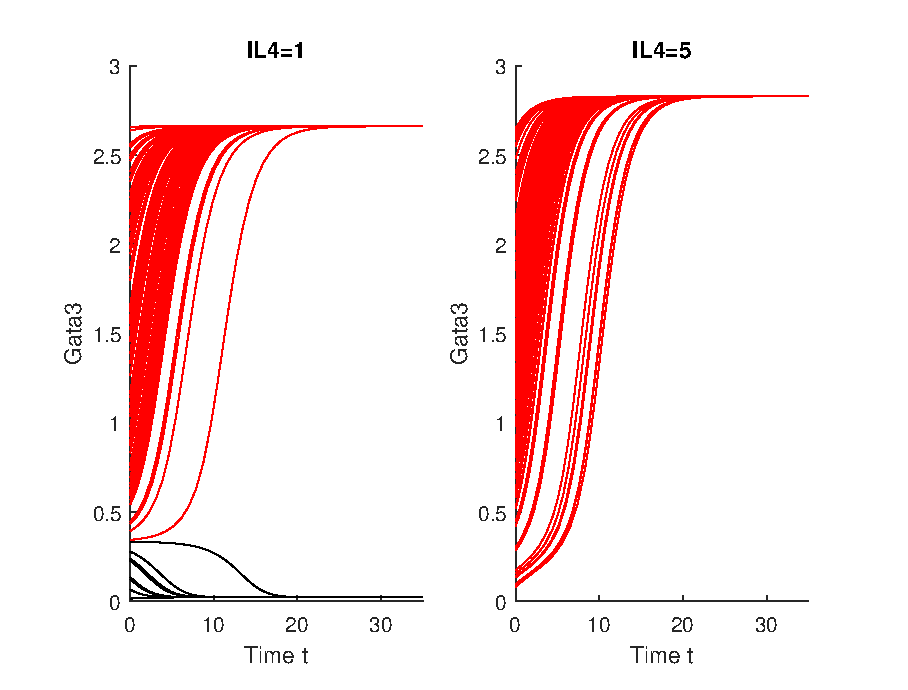
\includegraphics[scale=.5]{Gata3_t} 
  \caption{Integración numérica del modelo de \cite{Hofer2002}}
 \label{fig:Gata3_t}
\end{figure}



\subsection{Diagrama de bifurcación}





\begin{figure}[h!]
  \centering
 \includegraphics[scale=1]{GATA_model} 
  \caption{Diagrama de bifurcación del modelo de \cite{Hofer2002} (threshold value is parameter dependent)}
 \label{fig:Gata3_model}
\end{figure}

\section{Sistemas hibridos analisis de puntos focales} 

\begin{enumerate}
\item Las variables lentas son $S(t)$ y $B(t)$, las cuales se asumen que cambian infinitamente más lento que $R(t)$ y $K(t)$. 
\item La tasa de producción de la barrera epitelial está dada en el modelo por un término de la forma $\phi  \left(1-B(t)\right)$, que presenta un sólo punto de equilibrio ($B_{ss}=1$), y por lo tanto, adaptación perfecta. Esta ecuación sin embargo no representa las regulaciones bioquímicas (feedback negativo) necesarios para producir este comportamiento.
\item Ver figura \ref{fig: Interface_model}(A). Los sistemas biestables generalmente presentan retroalimentación positiva y cooperatividad. Un ejemplo es el modelo de diferenciación de células T, analizado en la pregunta anterior (figura \ref{fig:Gata3_model}).
\item Monoestabilidad "sana", monoestabilidad "enferma", biestabiilidad y oscilaciones (figura  \ref{fig: Hybrid_system_behaviours})
\item  \verb|Generate_2D_Bifurcation_diagram_Hybrid_System_practica.m}|\item Simplemente hay que correr el código \verb|Example_Trajectories_4_Dynamic_Phenotypes.m| .. usa varias funciones auxiliares, pero lo esencial es que usa la \textit{función localizadora de eventos}.
\end{enumerate}


\begin{figure}[h!]
  \centering
 \includegraphics[scale=.75]{Hybrid_system_behaviours.eps} 
  \caption{     }
 \label{fig: Hybrid_system_behaviours}
\end{figure}


\begin{figure}[h!]
  \centering
 \includegraphics[scale=.75]{Interface_model.eps} 
  \caption{\cite{Dominguez-Huttinger2016a} 
     }
 \label{fig: Interface_model}
\end{figure}



\bibliographystyle{unsrt}

\bibliography{C:/Users/Elisa/Dropbox/Postdoc_2015/Literature/library}

\end{document}



